\chapter{Reinforcement Learning}

\label{ch:RL} 

\newcommand{\inlinecode}[1]{\colorbox{evenmorelightgray}{\lstinline[basicstyle=\ttfamily\color{black}]{#1}}}

%----------------------------------------------------------------------------------------
%	INTRO
%----------------------------------------------------------------------------------------
As the task at hand was not only to provide a reinforcement learning agent, but also to convert a game itself into something the agent can successfully play, In this chapter I will go into detail about reinforcement learning in general, giving insights on the specific approach chosen. The descriptions will be kept as general as possible at first, with detailed explanations following in the sections about specific algorithms.
%TODO: dass das auf nen model-free, active, ... Q-learner hinausläuft?
%[The sense of this chapter is to give an intro of MDPs and RL. It shall also go into enough details on how to specify an MDP such that an RL agent can learn on it, because a big part of  the work was exactly that. It’s supposed to end with SARSA and Q-learning as the two Ideas on how to perform RL]

%----------------------------------------------------------------------------------------
%	SECTION 1
%----------------------------------------------------------------------------------------
\section{Reinforcement Learning Problems}

Machine Learning can mainly be subdivided into three main categories: Supervised Learning, Unsupervised Learning, and Semi-supervised learning. The first deals with direct classification or regression using labelled data which consists of pairs of datapoints with their corresponding category or value. In unsupervised learning, no such label exists, and the data must be clustered into meaningful parts without any knowledge, for example by grouping objects by similarity in their properties.\\
In this thesis, a certain kind of semi-supervised learning will mainly be considered: \keyword{Reinforcement learning} (\textbf{RL}). In RL, instead of labels for the data, there is a \textit{weak teacher}, which provides feedback on actions performed by the learner.

\subsubsection{Markov Decision Processes} \label{ch:mdps}

RL can be understood by means of a decision maker (\keyword{agent}) performing in an \keyword{environment}. The agent makes observations in the environment (its input), takes actions (output) and receives rewards. In contrast to the classical ML approaches, in RL the agent is also responsible for exploration, as he has to acquire his knowledge actively. Thus, a reinforcement learning problem is given if the only way to collect information about the \keyword{underlying model} (the environment) is by interacting with it. As the environment does not explicitly provide actions the agent has to perform, its goal is to figure out the actions maximizing its cumulative reward until a training episode ends.
%"put very simply, the agent wants to repeat the actions that give the highest reward

In the classical RL approach, the environment is divided into discrete time steps. If that is the case, the environment corresponds to a \keyword{Markov Decision Process} (\textbf{MDP}). Formally, a MDP is a 5-tuple $\langle S, A, P, R, \gamma \rangle$, consisting of the following:\\
\begin{align*}
\mathcal{S} &- \text{\small set of states } s\in \mathcal{S}\\
\mathcal{A} &- \text{\small set of actions } a \in \mathcal{A}\\
P(s'|s, a) &- \text{\small transition probability function from state } s \text{\small ~to state } s’ \text{\small ~under action } a: \mathcal{S} \times \mathcal{A} \rightarrow \mathcal{S} \\
R(r|s, a) &- \text{\small reward probability function for action } a \text{\small ~performed in state } s: \mathcal{S} \times \mathcal{A} \times \mathcal{S} \rightarrow \mathds{R} \\
\gamma &- \text{\small discount factor for future rewards } 0 \leq \gamma \leq 1
\end{align*}

%dass wir eigentlich noch ne initial state distrubition haben, und dass für den reward gilt S x A -> |R
In general, both the state transition function and the reward function may be indeterministic, meaning that neither reward nor the following state are in complete control of the decision maker. Because of that, only expected values are examinable, depending on the random distribution of states. Given both $s$ and $s'$ however, the reward is assumed to be deterministic. I will refer to the actual result of a state transition at discrete point in time $t$ as $s_{t+1}$ and to the result of the reward function as $r_t$. If no point in time is explicitly specified, it is assumed that all variables use the same $t$.\\

\noindent While an \keyword{offline learner} receives the problem definition as input in the form of a complete MDP, where the only task left is to classify actions yielding high rewards from actions giving suboptimal results, the task for an \keyword{online reinforcement learning} agent is a lot harder, as it has to learn the MDP itself via trial and error. In the process of reinforcement learning, the agent will encounter states $s$ of the environment, performing actions $a$. The future state $s_{t+1}$ of the environment may be indeterministic, but depends on the history of previous states $s_0, .., s_t$ as well as the action of the agent $a_t$. It is assumed that the \keyword{Markov property} holds, which means that a state  $s_{t+1}$ depends only on the current state $s_t$ and currenct action $a_t$: $p(s_{t+1}|s_t,a_t) = p(s_{t+1}|s_0,a_0,..,s_t,a_t)$

Throughout interacting with the environment, the agent receives rewards $r$, depending on his action $a$ as well as the state of the environment $s$. In many RL problems, the full state of the environment is not known to the agent, and it only perceives an observation depending on the environment: $o_t := o(s_t)$\footnote{From now on, when the state of the environment is meant, it will be explicitly referred to as $s_e$, while $s$ is reserved for the agent's obvervation of the enviroment $o(s_e)$}. This is referred to as \keyword{partial observability}, and the corresponding decision process is a \keyword{partially observable MDP}. Additionally, the agent knows when a final state of the environment is reached, terminating the current training episode. For the agent, an episode therefore consists of observations, actions and rewards ($\mathcal{S} \times \mathcal{A} \times \mathds{R}$) until at time $t_t$ some terminal state $s_{t_t}$ is reached: $$Episode := \big((s_0, a_0, r_0), (s_1, a_1, r_1), (s_2,a_2,r_2), .., (s_{t_t}, a_{t_t}, r_{t_t})\big)$$
%A training example for the agent thus consists of the tuple  <o_t, a_t, r_t, o_{t+1}, t>. 

\subsubsection{Value of a state}
In the process of reinforcement learning, the agent tries to perform as well as possible in the previously unknown environment. For that, it uses an \mbox{action-policy $\pi$,} depending on some parameters $\theta$. The policy maps states to actions, which in the case of a \keyword{deterministic} policy leads to $\pi_\theta(s) = a$. Though a stochastic policy is possible, it will not be considered for now\footnote{It is obvious, that the result of both the reward function and the state transition function depend on $\pi$. To be explicit about that, I will refer to a reward dependent on $\pi$ as $r^\pi$ and a state transition dependent on $\pi$ as $s^\pi$. If state or reward depends on an explicit action instead, I refer to it as $r^a$ and $s^a$. Whenever not necessary for clarity, I will also drop $\pi$'s dependence on $\theta$.}. %TODO problem hier: es hängt ja von rho^pi ab... und r ist ja eindeutig given both states and the action... hmmm wie drücke ich das gut aus? :/
As the agent does not have supervised data on which actions are the ground truth, it must learn some kind of measure for the value of being in a certain state or performing a certain action. The commonly used measure for the value of a state when using policy $\pi$ can be calculated by the immediate reward this state gives, summed with the expected value of the discounted future reward the agent will archieve by continuing to follow its policy $\pi$ from this state on:
\begin{equation} \label{eq:valuedefinition}
	V^\pi(s_t) := \mathds{E}_{s\sim\rho^\pi} \left[ \sum_{t'=t}^{t_t} ( \gamma^{t'-t} * r^\pi_{t'} ) \right]
\end{equation}
As the future rewards depend on future states, it can only be talked about the expected value depending on the actual state distribution. This distribution depends on the agents policy, but may still be indeterministic\footnote{That is one of the reasons to discount future rewards: The agent cannot be fully sure if it actually reaches the states it strives for. Also, using the discounted reward hopefully helps making the agent perform good actions as quickly as possible.}. The discounted state visitation distribution, which assigns each state a probability of visiting it according to policy $\pi$, is denoted $\rho^\pi$. 

The actual, underlying value of a state $V^*(s)$ could accordingly be defined as the value of the state when using the best possible policy, which corresponds to the maximally archievable reward starting in state $s_t$:
\begin{equation*} 
	V^*(s_t) := max_\pi V^\pi(s_t)
\end{equation*}

While \keyword{passive learning} simply tries to learn the value-function $V^*$ without the need of action selection, an \keyword{active reinforcement learner} tries to estimate a good policy that can actually reach those high-value states. If the value of every state is known, then the optimal policy can be defined as the one archieving maximal value for every state of the MDP: \mbox{$\pi^* := argmax_\pi V^\pi(s) \forall s \in \mathcal{S}$}. Knowing what an optimal policy does, the definition of the value $V^\pi(s)$ \ref{eq:valuedefinition} can be written recursively as
\begin{align}
	V^\pi(s_t) &= \mathds{E}_{s\sim\rho^\pi} \left[  \sum_{t'=t}^{t_t} ( \gamma^{t'-t} * r^\pi_{t'} ) \right]  \nonumber \\
	&= r_t^\pi + \gamma * \mathds{E}_{s\sim\rho^\pi} \left[  \sum_{t'=t+1}^{t_t} ( \gamma^{t'-t} * r^\pi_{t'} ) \right]  \nonumber \\
	&= r_t^\pi + \gamma * V^\pi(s_{t+1}) \label{statebellman}
\end{align}
%again, dass r von pi abhängt wird nicht deutlich
This relation is known as the \keyword{Bellman Equation}, which allowed for the birth of dynamic programming\footnote{Dynamic programming is another solution strategy for MDPs. In contrast to RL however, it requires the complete MDP as input to find an optimal policy, which cannot be given in many relevant situations.}.
% TODO CITE HINZUFÜGEN!!!!!!!!
%https://en.wikipedia.org/wiki/Bellman_equation#The_Bellman_equation

\subsubsection{Value of an action}
While the definition of a state-value is useful, by itself it does not help an agent to perform optimally, as neither the successor function $P(s'|s,a)$, nor the reward function $R(r|s,a)$ is known to the agent. While so-called \keyword{model-based} reinforcement learning (also referred to as \keyword{Certainty Equivalence}) tries to learn both of those explicitly to reconstruct the entire MDP, \keyword{model-free} agents use a different measure of quality: the \keyword{Q-value}. It represents the expected value of performing action $a_t$ in a state $s_t$, afterwards following the policy $\pi$:
\begin{equation} \label{eq:1.2}
	Q^\pi(s_t,a_t) :=  \mathds{E}_{s\sim\rho^\pi} \big[ r_t^{a_t} + \gamma * V^\pi(s_{t+1}^{a_t}) \big]
\end{equation}
With the Q-value $Q^*$ of the optimal policy accordingly 
\begin{align*}
	Q^*(s_t,a_t) &=  \mathds{E}_{s\sim\rho^\pi} \big[ r_t^{a_t} + \gamma * V^*(s_{t+1}^{a_t}) \big] \\
	&= max_\pi Q^\pi(s_t,a_t)
\end{align*}

For the Q-value, the Bellman equation holds as well: If the correct Q-value under policy $\pi$, $Q^\pi(s_{t+1},a_{t+1})$, was known for all possible actions at time $t$, then the optimal action is the one maximizing the sum of immediate reward and corresponding Q-value. This is because of the definition of Bellman's \keyword{Principle of Optimality}, which states that ``\kern-2pt \textit{An optimal policy has the property that whatever the initial state and initial decision are, the remaining decisions must constitute an optimal policy with regard to the state resulting from the first decision}''  (quote \cite{bellman_dynamic_nodate}). Thanks to the principle of optimality, the value of our decision problem at time $t$ can be re-written in terms of the immediate reward at $t$ plus the value of the remaining decision problem at $t+1$, resulting from the initial choices:
\begin{equation} \label{bellman}
	Q^\pi(s_t,a_t) =  \mathds{E}_{s\sim\rho^\pi} \big[r_t^{a_t} + \gamma *  Q^\pi(s_{t+1},\pi(s_{t+1}))  \big]
\end{equation}

As the value of a state is defined as the maximally archievable reward from that state, the relation between $Q$ and $V$ can be expressed as
\begin{equation} \label{eq:QandV}
V(s_t) = max_{a_t} Q(s_t, a_t)
\end{equation}

\subsubsection{Quality of a policy}

Any agent's goal is to find a policy that can follow the trajectory of the state distribution with the highest expected reward. If the actual Q-value for each action of each state is known, then the optimal policy can be defined as the one taking the optimal action in each state:
\begin{equation}
	\pi^* = argmax_aQ^*(s,a) \forall s,a \in \mathcal{S} \times \mathcal{A}
\end{equation}
This policy guarantees maximum future reward at every state. Note however, that finding $argmax_aQ(s,a)$ is only easily possible if $\mathcal{A}$ is discrete and finite (more on that later). 

As for the actual performance of a policy, a useful measure is the \keyword{performance objective} $J(\pi)$, which stands for the cumulative discounted reward from the start state using the respective policy. To measure the performance objective, it is necessary to integrate over the whole state space $\mathcal{S}$ with each state $s$ weighted by its distribution due to $\pi$. As only non-stochastic policies are considered here, integration over the action space $\mathcal{A}$ is not necessary. The integral can, as shown by \cite{silver_deterministic_2014}, be expressed by the expectation of the value of states following the distribution $s\sim\rho^\pi$:
\begin{align}
	J(\pi) &= \int_\mathcal{S} \rho^\pi(s) V^\pi(s) ds \nonumber\\
	       &= \mathds{E}_{s\sim\rho^\pi} \big[V^\pi(s)] \nonumber\\
	       &= \mathds{E}_{s\sim\rho^\pi} \big[Q^\pi(s, \pi(s))] \label{eq:performance01}
\end{align}
%TODO dass das jetzt bei off-policy anders ist, da wir da differentiaten müssen zwischen policy der wir folgen und policy anhand derer wir evaluieren!!!!!!!


\noindent We assume for now that once an agent knows $Q^*$, it can simply follow the policy that always takes the action yielding the highest value for every state (the \keyword{greedy} policy)\footnote{in fact, the agent cannot act only according to the greedy policy, as it will need to \keyword{explore} the environment first. The problem of exploration will be considered later in this thesis.}. 

Thus, the goal of a model-free RL agent is to get a maximally precise estimate of $Q^*$. To do that, it does not need to explicitly learn the reward- and transition function, but instead can model the Q-function directly. In RL settings with a highly limited amount of discrete states and actions, the respective Q-function estimate can be specified as a lookup le, whereas for areas of interest, the function is estimated using a nonlinear function approximator. The agent's approximation of $Q^\pi$ will be denoted $\hat{Q}^\pi$. \\

\noindent Throughout exploration of the environment, the agent collects more information about it, continually updating its estimate $\hat{Q}^\pi$. For that, it uses samples from its episodes of interacting with the environment. % also s, a, r, s', a', t.... wie formulier ich das gut?

%----------------------------------------------------------------------------------------
%	SECTION 2
%----------------------------------------------------------------------------------------
\section{Temporal difference learning}
%TODO actually, its only TD learning if we're learning the VALUE-function

%die relevanten cites hier sind sutton1988 und watkins1989. Der proof is dayan1992... und sowieso bellman
%Reinforcement learning can solve Markov decision processes without explicit specification of the transition probabilities; the values of the transition probabilities are needed in value and policy iteration. In reinforcement learning, instead of explicit specification of the transition probabilities, the transition probabilities are accessed through a simulator that is typically restarted many times from a uniformly random initial state. Reinforcement learning can also be combined with function approximation to address problems with a very large number of states.

%The goal of a reinforcement-learning agent is to continually update its Q*-estimate, Qpi, such that it can follow the policy that always takes the action giving the highest cumulative reward. To update its Q-function, the agent can either use full pairs of State,action,reward,state,action-tuples (SARSA, source), or Q-learning (source).
%Temporal difference learning ist Sutton 1988 in ftp://mi.eng.cam.ac.uk/pub/reports/auto-pdf/rummery_tr166.pdf
%Q-learning is Watkins 1989 in ibidem

Throughout the process of reinforcement learning, the agent continually improves its estimates $\hat{Q}^\pi$ of $Q^\pi$. The loss of its current estimate could be seen as the squared difference $(\hat{Q}^\pi - Q^\pi)^2$, however, as the agent has no knowledge of $Q^\pi$, it needs some way of approximating it. For that, a Q-learning agent performs \keyword{iterative approximation}, using the information about the environment, to continually update its estimates of $Q^\pi$.
\noindent Using the recursive definition of a Q-value given in the Bellman equation \ref{bellman} allows for a technique called \keyword{temporal difference learning}\cite{sutton_learning_1988}: At time $t+1$, the agent can compare its estimate of the Q-function of the last step, $\hat{Q}^\pi(s_t, a_t)$, with a new estimate using the new information it gained from the environment: $r_{t+1}$ and $s_{t+1}$.  Because of the newly gained information from the underlying MDP, the new estimate will be closer to the actual function $Q^\pi$ than the original value:
\begin{align} 
	\hat{Q}^\pi(s_t,a_t) &= r_t + \mathds{E}_{s\sim\rho^\pi} \big[ \gamma * max_{a_{t+1}} \hat{Q}^\pi(s_{t+1},a_{t+1})  \big]\\
	                     &\approx r_t + \gamma * r_{t+1} + \mathds{E}_{s\sim\rho^\pi} \big[ \gamma^2 * max_{a_{t+2}} \hat{Q}^\pi(s_{t+2},a_{t+2})  \big] \label{bellmanmal2}
\end{align}

%Q^\pi(s_t,a_t) :=  \mathds{E}_{s\sim\rho^\pi} \big[ r_t^{a_t} + \gamma * V^\pi(s_{t+1}^{a_t}) \big]

Keeping in mind that $\hat{Q}^\pi$ is only an estimator of the $Q^\pi$-values of the underyling model, it becomes clear that equation \ref{bellmanmal2} is closer to the actual $Q^\pi$, as it incorporates more information stemming from the model itself. 

In temporal difference learning, the mean-squared error of the \keyword{temporal difference} from this Bellman equation, $r_t + \gamma * Q(s_{t+1},a_{t+1}) - Q(s_t,a_t)$, gets minimized via iterative approximation. Even though $r_t + \gamma * \hat{Q}^\pi(s_{t+1},a_{t+1})$ also uses an estimate, it contains more information from the environment, and is thus a \textit{more informed guess} than $\hat{Q}^\pi(s_s,a_s)$. That makes it reasonable to substitute the unknown $Q^\pi(s_{t+1},a_{t+1})$ by $\hat{Q}^\pi(s_{t+1},a_{t+1})$.

\noindent It is noteworthy, that each update of the Q-function using the temporal difference will affect not only the last prediction, but all previous predictions.

%Q^*(s_t,a_t) &= \mathds{E}_S \big[ r_t^{a_t} + \gamma * V^*(s_{t+1}^{a_t}) \big]\\
%% &= r_t^{a_t} + \gamma * \Big( r_{t+1}^{a_\pi} + \gamma * V^\pi(s_{t+2}^{a_\pi})\Big) \\
%&\approx \mathds{E}_S \big[ r_t^{a_t} + \gamma * V^\pi(s_{t+1}^{a_t}) \big] = \mathds{E}_S \big[ r_t^{a_t} + \gamma * \hat{Q}^\pi(s_{t+1}^{a_t},a_{t+1}) \big]

%dass The only difference between maxa Q(s, a) and maxa'Q(s',a') is the immediate reward and the discount factor, and this is the only thing we update. If the received reward is higher than the expected reward, we will increase Q(s, a), or decrease it if our estimate was too high

% TODO sarsa ist sutton and barto 1998
\subsubsection*{\textsc{SARSA}}
The new knowledge about the environment can be incorporated in two different ways. For the first method, the agent samples a full tuple of $\langle s_t, a_t, r_t, s_{t+1}, a_{t+1} \rangle$ from its interaction with the environment, to then calculate the temporal difference error in non-terminal states as $ TD := (r_t + \gamma * \hat{Q}^\pi(s_{t+1}, a_{t+1})) - \hat{Q}^\pi(s_t, a_t)  $. This algorithm of calculating the temporal difference error is known as  \keyword{\textsc{sarsa}}, and it is an example of \keyword{on-policy} temporal difference learning. In on-policy learning, the agent uses its own policy in every estimate of the Q-value. If the policy of the agent is not stochastic, this method can however lead to it getting stuck in local optima.

\subsubsection*{Q-learning}

The \keyword{Q-learning} algorithm \cite{watkins_learning_1989} stands in contrast to \textsc{sarsa}. Q-learning does not need to sample the action $a_{t+1}$, as it calculates the Q-update at iteration $i$ using the best possible action in state $s_{t+1}$\footnote{A slight deviation from this is\keyword{double-Q-learning}, an architecture I will go into detail about later on.}. 

As the previous definition of Q-values was only correct in non-terminal states, a case differentiation must be introduced for terminal- and non-terminal states. In the following, $y_t$ will stand for the updated estimate of the Q-value at $t$, sampling the necessary states, rewards and actions from interaction with the environment, almost resulting in the formula found in \cite{mnih_human-level_2015}. To express its dependence on the policy $\pi$, it will be superscripted:
\begin{equation} \label{eq:ycases}
	y_t^\pi = \begin{cases} 
		r_t & \text{if } t = t_t\\
		r_t + \gamma * max_{a'} \hat{Q}^\pi( s_{t+1}, a') & \text{otherwise}
\end{cases}
\end{equation}
The temporal difference error for time $t$ is accordingly defined as 
\begin{equation}
TD_t := y_t^\pi - \hat{Q}^\pi(s_t, a_t)
%TD_t := \big( r_t + \gamma * max_{a_{t+1}}(\hat{Q}_i^\pi(s_{t+1}, a_{t+1}))\big) - \hat{Q}_i^\pi(s_t, a_t)
\end{equation}

A Q-learning agent must thus observe a snapshot of the environment, consisting of the following input: $\langle s_t, a_t, r_t, s_{t+1}, t+1==t_t \rangle$ (where the last element is the information if state $s_{t+1}$ was a terminal state). That information is then used to calculate the temporal difference error.

In very limited settings, using the above error straight away allows for the update-rule in simple Q-learners: Consider an agent, specifying its approximation of the Q-function (his \keyword{model}) with a lookup-table, initialized to all zeros. It is proven by \cite{watkins_technical_1992} that for finite-state Markovian problems with nonnegative rewards the update-rule for the Q-table (with $0 \leq \alpha \leq 1$ as the learning rate)
\begin{equation} \label{eq:qtable}
	\hat{Q}^\pi_{i+1}(s_t,a_t) \leftarrow \alpha * \Big(r_t^{a_t} + \gamma * \hat{Q}^\pi_i(s_{t+1}^{a_t},a_{t+1}) \Big) + (1-\alpha) * \hat{Q}^\pi_i(s_t,a_t)
\end{equation}
converges to the optimal $Q^*$-function, making the greedy policy $\pi^*$ optimal\footnote{Of course the agent will need some kind of exploration technique first, more on that later}. Note, that the same update rule as for the Q-function could be performed for the V-function.\\

In contrast to \textsc{Sarsa}, Q-learning is an \keyword{off-policy} algorithm, meaning that the policy it uses in its evaluation of the Q-value is not necessarily the one it actually uses: When calculating the temporal difference error, the agent considers Q-values $\hat{Q}^{\pi_{greedy}}(s,a)$, based on $\pi_{greedy}(s) = argmax_{a'}\hat{Q}(s,a')$, as better approximation of the real action-value function $Q^\pi(s,a)$. Therefore, it learns about $\pi_{greedy}$, which is to always take the action promising maximum value. Because following the deterministic $\pi_{greedy}$ does not allow for  \keyword{exploration}, this is not the policy the agent actually pursues. 

When using off-policy algorithms with $\pi$ as the policy we learn about and $\beta$ as the policy we act upon, our performance objective $J(\pi)$ (equation~\ref{eq:performance01}) must change, as it must incorporate that while the value of a state is calculated using our deterministic $\pi$, the distribution of states follows from stoachastic policy $\beta$: 
\begin{align} 
	J_\beta(\pi) &= \int_{\mathcal{S}} \rho^\beta(s) V^\pi(s) ds \nonumber\\
	&= \mathds{E}_{s\sim\rho^\beta} \big[Q^\pi(s, \pi(s)) \big] \label{eq:performance}
\end{align}\\

The process of reinforcement learning consists of two steps: \keyword{policy evaluation}, where the agent evaluates its current policy according to the knowledge gained from the environment, and based on that \keyword{policy improvement}. In the standard Q-learning considered here, those steps are interleaved, leading to a form of \keyword{generalized policy iteration}: the Q-learner learns its action value-function and its policy simultaneously. After updating its Q-function estimate via the temporal difference error, the agent updates its policy to be a \keyword{soft} version of the greedy policy $\pi_{i+1}(s) := argmax_{a'} Q^{\pi_i}(s,a') \forall s \in \mathcal{S}$, while keeping a mechanism allowing for exploration.  Learning with this approach is however generally limited: $argmax_{a'}Q(\cdot, a')$ can only easily be found in settings where the action space $\mathcal{A}$ is finite and discrete, as it requires a global maximization over all possible actions. In a later section, I will go into detail about another architecture which does circumvents those problems by splitting up policy evaluation and policy improvement explicitly.\\


As there are also relevant situations in which discrete actions $\mathcal{A} \subseteq \mathds{N}^n$ are sufficient, I will stick to those situations for now. Also in these circumstances, a Q-learner using tables as Q-function-approximator reaches its limits really fast, as the state space $\mathcal{S}$ may also be continuous or simply too big for a table to be useful. If that is the case, an update rule like in equation \ref{eq:qtable} becomes irrelevant quickly. Instead, a better idea is to use the definition of the temporal difference error to define a loss function, which is to be minimized throughout the process of RL. A commonly used loss-function is the \keyword{L2-Loss}, which allows for gradient descent, updating the parameters of the Q-function into the direction of the newly acquired knowledge. In this case, it may also be useful to calculate the loss of a batch of temporal differences simultaneously, which will be elaborated lateron in more detail. The L2-Loss for batch $batch$ with model-parameters $\theta_i$, making up the policy $\pi_{\theta_i}$ is thus defined as the following: 
\begin{equation} \label{l2loss}
	L_{batch}(\theta_i) := \mathds{E}_{s,a,r \sim batch} \Big[ \big( y_{batch}^{\pi_{\theta_i}} - \hat{Q}_{batch}^{\pi_{\theta_i}}(s, a)\big)^2 \Big]
\end{equation}







%sources so far:
%Heidemanns slides - check.
%meine eigene präsi - check. Wobei ich in der noch die erwartungswerte hab, und hier nicht..
%https://en.wikipedia.org/wiki/Markov_decision_process - check
%https://github.com/ahoereth/ddpg/blob/master/exploration/FrozenLake.ipynb  - check
%https://en.wikipedia.org/wiki/Reinforcement_learning
%https://en.wikipedia.org/wiki/Bellman_equation#The_Bellman_equation
%Valentins und melisas präsi
%Nature paper
%
%Medium post
%Russel, norvig
%Die originalen RL und Q-learn paper
%Meine und bennis präsi
%Report von valentin melisa und mir und benni

% TODO: Ich bin hier noch nicht auf exploration eingegangen... Und außerdem nicht auf actor-critic stuff oder policy gradients, kann ich also jetzt schon mit DQN kommen oder ist das viel zu früh?
% TODO: offensichtlich, die references. Mainly originales Qlearnpaper, was von bellman, originales reinforcementlearnpaper

%----------------------------------------------------------------------------------------
%	SECTION 3
%----------------------------------------------------------------------------------------
\section{Q-Learning with Neural Networks}

To understand this section, basic knowledge on how \keyword{Artificial Neural Networks} (\textbf{ANN}s) work and what they do is presupposed. Specifically, knowledge of \keyword{Convolutional Neural Networks} (\textbf{CNN}s)\cite{yann_lecun_gradient-based_1998}, mainly used in image processing, is required. As mentioned before, it is (in theory) not only possible to use a Q-table to estimate the $Q^\pi$-function, but any kind of function approximator. Thanks to the universality theorem, it is known that ANNs are an example of such\footnote{For a proof of the universality theorem, I refer to chapter 4 of Michael A. Nielsen's book ``\textit{Neural Networks and Deep Learning}'', Determination Press, 2015. The referred chapter is available at \url{http://neuralnetworksanddeeplearning.com/chap4.html}}. The defining feature of ANNs in comparison to other Machine Learning techniques is their ability to store complex, abstract representations of their input when using a \keyword{deep} enough architecture.

\subsection{Deep Q-learning} \label{ch:DQN}

\noindent The reason to use neural function approximators instead of a simple Q-table approach for reinforcement learning problems is easy to see: While for a Q-table the states and actions of the Markov Decision Process must be discrete and very limited, this is not the case when using higher-level representations. If the agent's observation of a state of the game is high-dimensional (like for example an image), the chance for an agent to observe the exact same observation twice is extremely slight. Instead, an Artificial Neural Network can learn a higher-level representation of the state, grouping conceptually similar states, and thus generalize to new, previously unseen states. It is no surprise that the success of \keyword{Deep-Q-Networks} started its journey shortly after the introduction of CNNs, which are able to learn abstract representations of similar images and by now used in countless Computer Vision Applications. \\%TODO: noch ne source?

\textit{Deep-Q-Network} (\textbf{DQN}) refers to a family of off-policy, online, active, model-free Q-learning algorithms for discrete actions using Deep Neural Networks. % I made it! I used all of those terms! :D
Using ANNs as function approximators for the agent's model of the environment requires a Loss function depending on the Neural Network parameters, specified by $\theta$. These weights correspond to the parameters of the $\hat{Q}$-function of the agent. As previously mentioned, this kind of Q-learning defines its policy straight-forward, depending on the $argmax_a$ of the Q-function. I will therefore replace the dependence of $\hat{Q}^\pi(s,a)$ on $\pi$ by a dependence on its parameters: $\hat{Q}(s,a;\theta_i)$. The update rule in Deep Networks depends on the gradient with respect to its loss, $\nabla_{\theta_i}L(\theta_i)$.  %ist so nicht ganz wie bei DQN, da da im linken teil der gleichung \theta^- = \theta_{i-1} verwendet wird.. check grad nur nicht warum ind er linken und nicht in der rechten hälfte
As the DQN-architecture only considers discrete actions, there is one change that can be made in the definition of the Q-function: instead of giving both the state $s$ and the action $a$ as input to the network, in DQNs only the state is input to the network, with the network returning a separate Q-value for each action $a \in \mathcal{A}$. This speeds up the inference, as one forward step is enough to calculate the Q-value of all actions in a certain state.\\

\noindent While there are attempts to use Artificial Neural Networks for Q-learning as early as 1994\cite{rummery_-line_1994}, some key components of modern Deep-Q-Networks were missing, leading to satisfactory performance only in very limited settings. In standard online RL tasks, the update step minimizing the loss specified in \ref{l2loss} is performed not for a batch, but for each time $t$ right after the observation occured to the agent. 
%in https://en.wikipedia.org/wiki/Markov_decision_process#CITEREFHoward1960 steht noch was zu policy iteration
%Deep Q Learning 
%While first ideas came up as early as 1993 (lin 1993 in ftp://mi.eng.cam.ac.uk/pub/reports/auto-pdf/rummery_tr166.pdf, ...
In those situations, the current parameters of the policy determine the next sample the parameters are trained on. It is easy to see, that those consecutive steps of MPDs tend to be correlated: It is very likely, that the maximizing action of time $t$ is similar to the one at $t+1$. Consecutive steps of an MDP are not representative of the whole underlying model's distribution. ANNs require independent and identically distributed samples, which is not given if the samples are generated sequentially. As shown by \cite{john_n._tsitsiklis_analysis_1997}, the update using gradient descent is prone to feedback loops and thus oscillation in its result, thus never converging to an optimal $Q^\pi$-function. 

It was not until \keyword{Deepmind}'s famous papers in 2013\cite{mnih_playing_2013} and 2015\cite{mnih_human-level_2015}, that those issues were successfully adressed. One important step when using ANNs instead of Q-tables is to perform stochastic gradient descent using minibatches. In every gradient descent step of the Neural Network, neither only the last temporal difference error $TD_t$ is considered (leading to oscillations), nor the entire sequence $TD_0, .., TD_{t_t}$ (because batch updates are not time-efficient in ANNs). Instead, as usual when dealing with ANNs, minibatches are sampled from the set of all observations. When performing the gradient descent step, the weights for the target $y_t$ are fixed, making the minimization of the temporal difference error a well-defined optimization problem (with clear-cut target values as in supervised learning) during the learning step.\\


\noindent The two important innovations introduced in the DQN-architecture were the use of a \keyword{target network} as well as the technique of \keyword{experience replay}, which in combination successfully solved the problem of oscillating and non-converging action-value functions, even though still no formal mathematical proof of convergence is given. %TODO: or is it by now? I could quote razvan pascanu here

\subsubsection*{Experience Replay}
%dass das auch data efficiency erhöht - alle 4 schritte wird ein 32er minibatch genommen, jedes wird mehrfach genutzt
As mentioned above, learning only from the most recent experiences biases the policy towards those situations, limiting convergence of the Q-function. To adress this issue, the DQN uses an experience replay memory: Every percept of the environment (the $\langle s_t, a_t, r_t, s_{t+1}, t+1==t_t \rangle$ - tuple) is added to a limited-size memory of the agent. When then performing the learning step, the agent samples random minibatches from this memory to perform learning on a maximally uncorrelated sample of experiences. In the original definition of DQN, those minibatches are drawn uniformely at random, while as of today, better techniques for sampling those minibatches are available\cite{schaul_prioritized_2015}, increasing the performance of the resulting algorithm significantly. %TODO dieses paper wirklich lesen und drauf eingehen, und am besten auch minimal coden, das ist superwichtig!

\subsubsection*{Target Networks}
During the training procedure, the DQN-algorithm uses a separate network to generate the target-Q-values which are used to compute the loss (eq. \ref{l2loss}), necessary for the learning step of every iteration. Intuitively speakin, this is necessary because the Q-values of the \keyword{online network} shift in such a way, that a feedback loop can arise between the target- and estimated Q-values, shifting the Q-value more and more into one direction. %TODO: das ist sehr unwissenschaftlich ausgedrückt und geht auf jeden Fall besser erklärt, using eine der vorhergegangenen 
To lessen the risk of such feedback loops, the DQN algorithm introduced the use of a second network for calculating the loss: the \keyword{target network}. This is only periodically updated with the weights of the online network used for the policy, which reduces the risk of correlations in the action-value $Q_t$ and the corresponding target-value $y_t$ (see equation \ref{eq:ycases}).

The use of these two techniques leads to the Q-learning update rule, using the loss as put forward in \cite{mnih_human-level_2015}:
\begin{equation} \label{qloss_target}
	L_i(\theta_i) = \mathds{E}_{\langle s_t,a_t,r_t,s_{t+1} \rangle \sim U(D)} \Bigg[\Big( r + \gamma * max_{a_{t+1}} \hat{Q}(s_{t+1}, a_{t+1}; \theta^-_i) - \hat{Q}(s_t,a_t;\theta_i) \Big)^2\Bigg]
\end{equation}
\begin{flushright}
	\scriptsize
	Where $i$ stands for the current network update iteration, $\theta_i$ for the current weights of the target network (updated every $C$ iterations to be equal to the weights of the online network $\theta_i$), $Q(\cdot,\cdot;\theta)$ for the Q-value dependend on a ANN using the weights $\theta$, $\mathds{E}[\cdot]$ for the expected value in an indeterministic environment, D for the contents of the replay memory of length $\lvert D \rvert$ containing $\langle s_t,a_t,r_t,s_{t+1} \rangle$-tuples, and $U(\cdot)$ for a uniform distribution.
\end{flushright}
As is the case with the experience replay mechanism, the usage of a target network was improved as well -- modern algorithms do not perform a hard update of the target network every $C$ steps, but instead perform \keyword{soft target network updates}, where every iteration, the weights of the target network are defined as $\theta^-_i := \theta_i * \tau + \theta^-_i * (1-\tau)$ with $0 < \tau \ll 1$, first introduced in \cite{lillicrap_continuous_2015}. This improves the stability of the algorithm even more.\\

As a pseudocode for the DQN-architecture is already stated in the corresponding paper \cite{mnih_human-level_2015}, listing it again here would be superflous. Instead, I try to compare the pseudocode with the code of my actual implementation using Python and Tensorflow in appendix~\ref{ap:dqn}. In the first two pages of the appendix, the necessary definitions of agent and network structure are introduced, before in page~\pageref{ap:dqn_comparison} there is the actual comparison between the pseudocode and its correspondences in the actual code, namely the \inlinecode{\_\_init\_\_}, \inlinecode{inference} and \inlinecode{q\_learn}-functions of the model-class. Note that the blue lines of the pseudocode correspond to difference from the original DQN in favor of later improvements.

\subsection{Double-Q-Learning}
It is well known that Q-learning tends to ascribe unrealistically high Q-values to some action-state-combinations. The reason for this is, that to estimate the value of a state $s_j$ it includes a maximization step over estimated action values $Q(s_j,a)$ , where naturally, overestimated values are preferred over underestimated values. 
It is not possible that Q-value-estimates are completely precise: estimation errors can occur due to environmental noise, inaccuracies in function approximation (consider a flexible ANN trained on only a small sample so far - the ANN will overfit by covering all samples precisely. This overfitting leads to steep curves, over- or underestimating many values in between) and many other issues. Because Q-learning uses the maximum Q-value of state $s_{j+1}$ in every estimate of the value of state $s_j$, only those estimates are propagated where the noise of the estimation is in a positive direction. Because of that, state $s_{j-1}$ will have the accumulated upward noise from both state $s_j$ and $s_{j+1}$, and so forth. This leads to unrealistically high action-values. While this would not constitute a problem if all Q-values would be uniformly overestimated, \cite{van_hasselt_deep_2015} showed that its very likely that the Q-value $Q(s_j,a)$ for only some actions $a$ is overestimated -- which changes the result of the $argmax_a$ operation and thus leads to biased policies. They also show that the drop in DQN performance correlates with this overestimation of actions.\\

The solution suggested by \cite{van_hasselt_deep_2015} is called \keyword{Double-Q-learning}. In its original definition without using Neural Networks as function approximators, a double-Q-learner learns two value functions in parallel, by letting each experience update only one of the two value functions at random. For each update then, one function is used to determine the greedy policy, while the other is used to determine the value of this policy\footnote{\textit{``In DoubleQ, we still use the greedy policy to select actions, however we evaluate how good it is with another set of weights''}. The intuition behind that is, that the probability of both value-functions always over-estimating the same actions is basically zero.}. The authors proved that the lower bound for the overestimation of action-value, $max_{a'}Q^\pi(s,a') - V^*(s)$, is $>0$ for the standard Q-learning update rule, whereas it is $0$ in the case of DoubleQ. Additionally they showed that these overestimations are indeed harmful by showing the superiority of a DoubleQ-learner in comparison with a normal Q-learner.\\

\keyword{Deep-Double-Q-Learning} (\textbf{DDQN}) takes the Double-Q idea to the existing framework of Deep-Q-learning: Overestimations are reduced by decomposing the $max$-operation into \keyword{action selection} and \keyword{action evaluation}. Instead of introducing a second value function, DDQN re-uses the target-network of the DQN architecture in place of the second value function. Although online network and target network are not fully decoupled, experiments showed that it provides a good candidate for independent action evaluation, without the need of additional functions. The technique of DDQN is thus to still use the online network to choose an action (evaluate the greedy policy according to the online network), but the target network to generate the target Q-value for that action (to estimate its value, instead of the max-operation in DQN). As shown by \cite{van_hasselt_deep_2015}, DDQN improves over DQN both in terms of value accuracy and in terms of the actual quality of the policy. 

When using Double-Q-Learning, the target-value of the calculation of the temporal difference error ($y_t$ from equation~\ref{eq:ycases} must thus be re-defined as 
\begin{equation}
		y_t^\pi = \begin{cases} 
	r_t & \text{if } t = t_t\\
	r_t + \gamma * Q(s_{t+1}, argmax_{a'} Q($  $s_{t+1}, a'; \theta_i); \theta_i^-) & \text{otherwise} 
	\end{cases} %  max_{a_{t+1}} \hat{Q}^\pi( s_{t+1}, a_{t+1})
\end{equation}

It can be seen in appendix~\ref{ap:dqn} how small the actual change to normal DQN is: The only difference is the usage of the target network in line~\ref{sourcecode_ddqn} (marked in blue).

\subsection{Dueling Q-Learning}

In many situations encountered during Q-learning, the value of all possible actions $a_t$ in a state $s_t$ is almost equal. Consider a simulated car, driving with full speed towards a wall, already so close that breaking or steering can't stop the car from driving into the wall. As all actions will end in the episode will end by the car hitting the wall, all actions will have roughly the same Q-value. 

The idea of the \keyword{dueling architecture}\cite{wang_dueling_2015} for DQN is to learn the action-state-value function more efficiently. For that, it splits up the Network into a \keyword{value stream} and separate \keyword{advantage streams}. As mentioned earlier, though the ANN resembles the $\hat{Q}(s,a)$-function, the actions are not input to the network, but instead it outputs $|\mathcal{A}|$ Q-values, one for each action. A \keyword{Dueling Double Deep-Q-Network} (\textbf{DDDQN}) works by splitting an early layer of its corresponding network in half. One of the resulting streams is the value-stream, which results in one value, intuitively corresponding to the value ($\hat{V_{s_t}}$) of a state $s_t$, irrespective of the action that can be taken in this state. The other stream is  the advantage stream, which has as output $|\mathcal{A}|$ values, standing for the \keyword{Advantage} ($A$) of taking a certain action in this state -- it can be seen as a relative measure of the importance of each action. The relation between $Q$, $V$ and $A$ is the following:
\begin{equation*}
	Q(s,a) = V(s) + A(s,a)
\end{equation*}
In the very last layer of the ANN those two streams are combined again, so that a DDDQN also outputs one Q-value for each action. Thanks to this, any DDQN can be transformed into a DDDQN by simply changing the structure of the used ANN. It is important to mention however, that the last layer can't simply calculate $V(s) + A(s,a)$ -- If that was done, then the network could simply set the V-stream to a constant, negating any advantage gain in splitting them up in the first place. However, as explained in equation~\ref{eq:QandV}, it holds that $argmax_{a'}Q(s,a') = V(s)$ -- when using deterministic policies, than the value of the state corresponds to the Q-value of the best action that can be taken in this state. Therefore, it must be the case that the $argmax$-action has an advantage of zero. This can be used to calculate the $Q(s,a)$ using the value-stream and the advantage-stream according to the following equation (where $\theta$ corresponds to the shared weights, $\theta^A$ to the weights specific to the advantage-stream and $\theta^V$ to those specific to the value-stream):
\begin{equation*}
	Q(s,a; \theta, \theta^A, \theta^V) = V(s; \theta, \theta^V) + \big( A(s,a; \theta, \theta^A) - max_{a'}A(s,a',\theta, \theta^A) \big)
\end{equation*}
Actually, during testing it turned out that normalizing the advantage not with respect to the best action, but with respect to the average of all actions, $\frac{1}{|\mathcal{A}|} \sum_{a'} A(s, a'; \theta, \theta^A)$ lead to better stability. By splitting up into separate advantage- and valuestream and combining the two streams in a fully-connected layer using the formula stated above, the authors archieved far better performance then their predecessor, DDQN, on the same dataset \cite{wang_dueling_2015}.\\

The reason to split into two streams is obvious: In the learning step of a DQN, the derivative is taken with respect to difference in the expected Q-value of an action and the better estimate of that Q-value. In normal DQNs, the network can thus only update the parameters responsible for one of its outputs. A DDDQN learns more effectively, as it learns a shared value of multiple actions: A temporal difference in one Q-value likely changes the value-stream of the network, which also changes the Q-value of other actions. Thanks to this, learning generalizes better across actions, without any changes to the underlying reinforcement learning algorithm. As shown by the authors \cite{wang_dueling_2015}, the difference is especially drastic in situations where many actions have similar outcomes.\\


In appendix~\ref{ap:dqn}, I listed an exemplary source code of the implementation of an agent using python and tensorflow. The agent stands alone without an environment, and some crucial parts of it, like an implementation of its memory, are missing. However, all aspects mentioned in the previous sections are found in it, which is the algorithm of the actual Q-learning as described above and in \cite{van_hasselt_deep_2015}, as well as the computation graph of the network using precisely the DDDQN-architecture as described above and in \cite{wang_dueling_2015}. The last page of it (page~\pageref{ap:dqn_comparison}) consists of a comparison of the Pseudocode of the DDDQN (as found in \cite{mnih_human-level_2015}, with the changes from \cite{van_hasselt_deep_2015} and \cite{lillicrap_continuous_2015} incorporated in and marked blue), where each line of the pseudocode (to the left) corresponds precisely to the respective line of the actual python-code (to the right).


%\subsection{Using Recurrent Networks}

%----------------------------------------------------------------------------------------
%	SECTION 4
%----------------------------------------------------------------------------------------

\section{Policy Gradient Techniques}

\keyword{Policy Gradient} (\textbf{PG}) techniques are in principle a far more straight-forward approach to reinforcement learning than temporal difference-methods like Q-learning. The idea behind PG techniques is really simple: The policy $\pi_\theta(a|s) = \mathds{P}[a|s;\theta]$ of an agent is explicitly modeled using a differentiable function approximator, like a neural network with weights $\theta$. There is no need  to approximate the value-function of states or actions explicitly. The quality of the policy is again measured by its performance as in equation~\ref{eq:performance}. 

Before continuing to explain PG techniques, it makes sense to define another measure of the quality of an action: The \keyword{advantage}. The advantage will be what PG methods optimize for, and it can be defined analogously to the value of a state in equation~\ref{eq:valuedefinition}, with the difference that this time, as we do not explicitly model the value of following states, we can only calculate it after having measured all of the respective rewards from the environment:
\begin{equation}
	 A_t := \sum_{t'=t}^{t_t} ( \gamma^{t'-t} * r_{t'} ) 
\end{equation}
To use the policy gradient, the agent must calculate the advantage of every state it visited so far, to then set this advantage as the gradient of the output of its policy function of the corresponding state, to then train the network using backpropagation with respect to this gradient. If the reward is positive, gradient \textit{ascent} will make the network more likely to produce this action in this state, and if the gradient was negative, it will lead to gradient \textit{descent}, discouraging the network to repeat this action in the given state. Thus, the network will learn to repeat actions giving high rewards and to avoid those with negative rewards.

This may sound unintuitive at first, because there is no specific loss function the ANN can optimize for. However in fact, using the gradient with respect to the advantage corresponds to the loss $\sum_t A_t~log~p(a_i|s_i)$ -- If $A_t$ is positive, we want to increase the probability of action $a_t$ for state $s_i$, and decrease it otherwise.\\

\noindent The main problem of purely using this approach is however the huge amount of exploration that is needed -- the agent does not have any knowledge about what states are good or bad, but only increases the probability of individual actions that turned out to have a good score. Because of this, it can find good policies only by chance, after millions of iterations. If the agent knew the value of a state, it could optimize its policy in the direction of actions that it knows produce a high-valued state. For that, the policy network must get the gradient information of the action from something estimating this value-function, giving rise to \keyword{actor-critic architectures}.

\subsection{Actor-Critic architectures}

The technique introduced in the previous sections is a direct adaption of the Q-learning algorithm \cite{sutton_learning_1988}\cite{watkins_learning_1989}, adapted for higher-level function approximators. Standard Q-learning is a kind of \keyword{generalized policy iteration}, where the policy evaluation and policy improvement happen in the same step. The algorithm learns via temporal differences the state-action value $Q^{\pi_{greedy}}(s,a)$ for the states it encountered with its current policy $\pi$. It then updates $\pi$ to a soft version of that greedy policy: $\pi_{i+1}(s) := soft(argmax_a Q^{\pi_{greedy}}(s,a) \forall s \in \mathcal{S})$, where the $soft$-function ensures appropriate exploration. Learning the Q-function and the policy simultaneously is however generally limited: $argmax_aQ(\cdot, a)$ can only easily be found in settings where the action space $\mathcal{A}$ is finite and discrete, as it requires a global maximization over all possible actions. While discretizing the action space is possible, it gives rise to the \keyword{curse of dimensionality}, especially when the discretization is fine grained. An iterative optimization process like the $argmax$-operation would thus likely be intractable.\\


\noindent However in a lot of scenarios, the action space is not discrete, but continuous: \mbox{$A \subseteq \mathds{R}^n$}. In such situations, the alternative is to move the policy into the \textit{direction of the gradient of Q}. For that, it is necessary to model the policy explicitly with another function approximator. This gives rise to \keyword{actor-critic} architectures, where both policy and Q-function are explicitly modeled: The \keyword{critic} corresponds again to a Bellman-function-approximator, using temporal differences to estimate the action-value $Q^\pi(s,a)$\footnote{In that, it corresponds precisely to the previous approach. However, as we now allow for a continuous action-space $\mathcal{A}$, the network cannot return multiple Q-values at once, for each action $a \in \mathcal{A}$. Instead, the actions must also be inputs to the critic, which then outputs one $Q(s,a)$-value.}. In contrast to the previous approach however, the policy is now explicitly modeled by the \keyword{actor}. In the case of a stochastic policy, it would be represented by a parametric probability distribution $\pi_\theta(a|s) = \mathds{P}[a|s;\theta]$, however here we only consider the case of deterministic policies $a = \pi_\theta(s)$, which takes the necessity of averaging over all possible actions when calculating its performance objective according to equation~\ref{eq:performance01} or equation~\ref{eq:performance}. Note however, that using deterministic policies will (again) lead to the necessesity of off-policy algorithms, as a purely deterministic policy does not allow for adequate exploration of state-space $\mathcal{S}$ or action-space $\mathcal{A}$. Thus, to measure the performance of our policy, we must use function \ref{eq:performance}, which averages over the state distribution of our behaviour policy $\beta \neq \pi$. 

To train both actor and critic, actor-critic algorithms rely on a version of the \keyword{policy gradient theorem}, which states a relation between the gradient of the policy and the gradient of its performance function. The idea behind actor-critic policy gradient algorithms is accordingly to adjust the parameters $\theta$ of the policy in the direction of the performance gradient $\nabla_{\theta}J(\pi_\theta)$, as moving uphill into the direction of the performance gradient corresponds to maximizing the global performance of the policy\footnote{The original policy gradient, introduced in \cite{sutton_policy_2000}, assumes on-policy learning with a stochastic policy. However, to derive the stochastic policy gradient, one must integrate over the whole action-space, making its usage less efficient and requiring more training than the DPG, introduced here.}. The DPG technique is the policy gradient analogue to Q-learning: It learns a deterministic greedy policy in an off-policy setting, following a trajectory of states due to a noisy version of the learned policy.

\subsubsection{Deterministic Policy Gradient}

The idea in the \keyword{Deterministic Policy Gradient} (\textbf{DPG}) technique is to use a relation between the gradient of the (deterministic) policy (represented by the actor), and the gradient of the action-value function Q. The existance of a relation is easy to see, because as introduced in equation~\ref{eq:performance}, the performance of our policy $\pi$ is measured using Q. 

The \keyword{off-policy deterministic policy gradient theorem}, put forward in \cite{silver_deterministic_2014}, states the following relation between the gradient of the performance objective of a policy $J(\pi)$ (see equation \ref{eq:performance}) and the gradients of the policy-function $\pi$ and the action-value function $Q$. 
\begin{align}
	\nabla_{\theta}J_\beta(\pi_\theta) &\approx \int_{\mathcal{S}} \rho^\beta(s) \nabla_\theta \pi_{\theta}(a|s)Q^\pi(s,a) ds \nonumber \\
	    &= \mathds{E}_{s\sim\rho^\beta} \Big[ \nabla_\theta \pi_\theta Q^\pi \big(s,\pi_\theta(s)\big)   \Big] \nonumber \\
		&= \mathds{E}_{s\sim\rho^\beta} \left[  \nabla_\theta \pi_{\theta}(s) \nabla_a Q^\pi(s,a) \big|_{a=\pi_\theta(s)} \right]  \label{eq:dpg}
\end{align}
\begin{flushright}
	\small There are two important things about this relation: first, it can be seen that the policy gradient does not depend on the gradient of the state distribution. Second, the approximation drops a term that depends on the action-value gradient, $\nabla_{\theta} Q^\pi(s,a)$. Since the position of the optima are however preserved, the term can be left  out, making the approximation no less useful. Both claims are shown in \cite{silver_deterministic_2014}.\\ 
\end{flushright}

\noindent The practical implication of this relation is the following:\\
\noindent When updating the policy, its parameters $\theta_{i+1}$ are updated in proportion to the gradient $\nabla_{\theta}J(\pi_\theta)$. In practice, each state suggests a different gradient, making it necessary to take the expectation w.r.t. the state distribution $\rho^\beta$: 
\begin{equation*}
	\theta_{i+1} = \theta_i + \alpha * \mathds{E}_{s\sim\rho^\beta} \big[ \nabla_{\theta}J(\pi_\theta) \big]
\end{equation*}

The deterministic policy gradient theorem (\ref{eq:dpg}) shows that to improve the performance of the policy, it makes sense to move it into the direction of the gradient of Q, where the gradient of Q can be decomposed into the gradient of the action-value with respect to the actions, and the gradient of the policy with respect to its parameters:
\begin{equation*}
	\theta_{i+1} = \theta_i + \alpha * \mathds{E}_{s \sim \rho^\beta} \left[ \nabla_\theta \pi_{\theta}(s) \nabla_a Q^{\pi_i}(s,a) \big|_{a=\pi_\theta(s)} \right]
\end{equation*} 
In other words, to maximize the performance of the policy, one can re-use the gradient of those actions leading to maximal Q-values. In practice, the true function $Q^\pi(s,a)$ is unknown and must be estimated.\\

\noindent The off-policy deterministic actor-critic algorithm learns a deterministic target policy $\pi_\theta(s)$ from trajectories generated by an arbitrary stochastic policy, $\beta(a|s) = \mathds{P}[a|s]$. For that, it uses an actor-critic arcitecture: The critic estimates the Q-function using a differentiable function approximator, using Q-learning as explained in the sections above, with the weights specified as $w$. The actor updates the \textit{policy} parameters $\theta$ in the direction of the gradient of Q (instead of maximizing it globally as in the sections above\footnote{\textit{``The critic estimates the action-value function while the actor ascends the gradient of the action-value-function''} (quote \cite{silver_deterministic_2014})}. Note that for the update of the policy parameters, only the gradient w.r.t. the weight of the actions as input of the Q-functions are relevant, not the trained weights of the approximator $Q^w$ itself. Figure~\ref{fig:actorcritic} visualizes the idea behind the algorithm graphically.
\begin{figure}[h]
	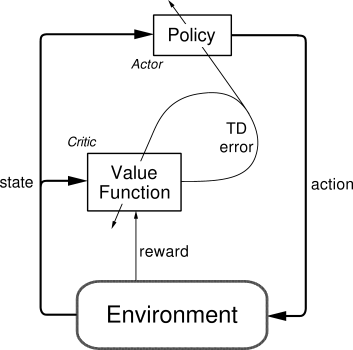
\includegraphics[width=.4\textwidth]{sutton-ac.png}
	\centering
	\caption{The actor-critic architecture. Reprinted from \cite{richard_s._sutton_reinforcement_1998}.}
	\label{fig:actorcritic}
\end{figure}

\noindent Using the above knowledge, one can derive the \keyword{off-policy deterministic actor critic} algorithm. In the first step of this algorithm, the critic calculates the temporal difference error to update its own parameters like in previous sections, and then the actor updates its parameters in the direction of the critic's action-value gradient:
\begin{align}
	TD_i    &= \mathds{E}_{s,a,r} \left[ \big( r_t + \gamma * Q^{w_i}(s_{t+1}, \pi_{\theta}(s_{t+1})) \big) - Q^{w_i}(s_t, a_t) \right] \label{eq:td_dpg}\\
	w_{i+1} &= \mathds{E}_{s,a} \left[  w_i + \alpha_w * TD_i \nabla_w Q^w(s_t, a_t) \right] \label{eq:critic_dpg} \\
	\theta_{i+1} &= \mathds{E}_{s,a} \left[ \theta_i + \alpha_\theta * \nabla_\theta \pi_\theta(s_t) \nabla_a Q^w(s_t,a_t) \big|_{a=\pi_\theta(s)} \right] \label{eq:actor_dpg}
\end{align}
\begin{flushright} \small With $\alpha_w$ and $\alpha_\theta$ as the learning-rates of the critic and the actor, respectively. \end{flushright}

As stated by \cite{silver_deterministic_2014}, these algorithm may have convergence issues in practice, due to a bias introduced by approximating $Q^\pi(s,a)$ with $Q^w(s,a)$. It is thus important, that the approximation $Q^w(s,a)$ is \keyword{compatible}, preserving the true gradient $\nabla_a Q^\pi(s,a) \approx \nabla_a Q^w(s,a)$. This is the case when the gradients are orthogonal, and $w$ minimizes $MSE(\theta,w)$. However, the necessary conditions are approximately fulfilled when using a differentiable critic that finds $Q^w(s,a) \approx Q^\pi(s,a)$.


\subsubsection*{Deep DPG}

The \keyword{Deep DPG Algorithm} is an off-policy actor-critic, online, active, model-free, deterministic policy gradient algorithm for continous action-spaces. The basic idea behind \keyword{Deep DPG} (\textbf{DDPG})\cite{lillicrap_continuous_2015} is to combine the ideas of the DQN (section \ref{ch:DQN}) with the architecture and learning rule using the deterministic policy gradient. For that, they also use parameterized deterministic actor function $\pi_\theta(s) = a$, as well as a critic function $Q^w(s,a)$. As the algorithm is also off-policy, it will learn the policy $\pi_theta$, while following a trajectory arising through another, stochastic policy $\beta$. This policy will again be a \textit{soft} version of the learned policy $\pi$ that allows for adequate exploration: $\beta := soft(\pi)$.

The update of the critic is performed analogously to the Q-value approximator in the Deep-Q-Network architecture. A minibatch of $\langle s_t, a_t, r_t, s_{t+1}, t==t_t \rangle$-tuples is sampled from a replay memory of limited size, to then perform Q-learning via temporal differences (see \ref{l2loss} and \ref{qloss_target}). An obvious difference to the Q-learning in the above sections is however, that not the greedy $argmax_{a'}Q(s,a')$-policy is used in the determination of the targetvalue, but the agent's own parameterized policy $\pi_\theta(s)$. Just like in Deep-Q-Learning, it is necessary to use target networks to ensure convergence of Q -- in fact, Lillicrap et. al. \cite{lillicrap_continuous_2015} were the first to use the previously mentioned soft target updates.

The update of the actor then follows the deterministic policy gradient theorem from equation~\ref{eq:dpg}: Its estimation of the policy gradient bases on the minibatch-samples used in the critic. For that, it calculates the expectation of the action-gradients it adopted from the critic network. This expectation is an approximation of its policy gradient, allowing the actor to perform a stochastic gradient ascent step to optimize its performance objective.

In practice, it turned out that the usage of target networks for both actor and critic is necessary to ensure stability of the algorithm, such that in practice, there are four different networks: the actors $Q(s,a;\theta^Q)$ and $Q(s,a;\theta^{Q^-})$ as well as the critics $\pi(s;\theta^\pi)$ and $\pi(s;\theta^{\pi^-})$. Incorporating all those changes leads to the following pseudocode snipplet of the agent's learning step, adopted from \cite{lillicrap_continuous_2015}: \\

\noindent Target-value of the critic:
\begin{equation} \label{eq:y_ddpg}
	y_t := \begin{cases} 
	r_t & \text{if } t = t_t\\
	r_t + \gamma * Q\big(s_{t+1}, \pi(s_{t+1};\theta^{\pi^-});\theta^{Q^-} \big)  & \text{otherwise} 
	\end{cases} %  max_{a_{t+1}} \hat{Q}^\pi( s_{t+1}, a_{t+1})
\end{equation}
\noindent Loss the critic minimizes:
\begin{equation} \label{eq:loss_ddpg}
	L_i(\theta^\pi_i) := \mathds{E}_{\langle s_t,a_t,r_t,s_{t+1} \rangle \sim U(D)} \Big[\Big( y_t - Q(s_t,a_t;\theta^Q) \Big)^2\Big]
\end{equation}
\noindent Sampled policy gradient the actor maximizes for:
\begin{equation} \label{eq:actor_ddpg}
	\nabla_{\theta^\pi}J_\beta(\pi_\theta) \approx \mathds{E}_{\langle s_t,a_t,r_t,s_{t+1} \rangle \sim U(D)} \Big[ \nabla_a Q(s_t,\pi(s_t);\theta^Q) \nabla_{\theta^\pi} \pi(s_t;\theta^\pi) \Big]
\end{equation}
The correspondences of this ANN implementation and the correspondences of the general definitions can easily be seen: Equations~\ref{eq:y_ddpg} and \ref{eq:loss_ddpg} correspond to definitions \ref{eq:td_dpg} and \ref{eq:critic_dpg}, whereas equation~\ref{eq:actor_ddpg} corresponds to equation~\ref{eq:actor_dpg}.\\

For a complete code of the DDPG-implementation, I refer to appendix~\ref{ap:ddpg}. Analogously to the DQN-agent, an exemplary source code of the implementation of an agent with a DDPG-model can be found there, using python and tensorflow. The agent stands alone without an environment, and some crucial parts of it, like an implementation of its memory, are missing. On page \pageref{ap:ddpg_comparison}, there is again a comparison of the pseudocode (as provided in \cite{lillicrap_continuous_2015}) and the correspondences in actual-python code, where each line of the pseudocode (to the left) corresponds precisely to the respective line of the actual python-code (to the right).


%----------------------------------------------------------------------------------------
%	SECTION 5
%----------------------------------------------------------------------------------------

\section{Exploration techniques}

There is one main difference between supervised learning and reinforcement learning, which I mentioned right at the beginning of this chapter: in RL, the only way to collect information about the environment is by interacting with it. In supervised learning it is no problem to shuffle the dataset beforehand, giving the learner i.i.d. samples, which are sure to be representatitive about the dataset. In RL however, this is not possible: Consider the situation where the agent drives a car around a track -- as long as the agent doesn't drive the car well enough, it will probably not reach high speeds, and will thus learn nothing about situations in which it drives at high speeds. Another problem which was also mentioned before is that so far, only deterministic policies $\pi(s) = a$ were considered. It is obvious that in practice, purely using deterministic policies leads to a complete lack of \keyword{exploration} of the state space $\mathcal{S}$ of the MDP: Once the agent found one path to a terminal state, it will continue \keyword{exploiting} this path, which almost gurantees a suboptimal solution. In order to explore the full state space instead of sticking with the first local optimum found, a stochastic, non-greedy policy is necessary.

The two algorithms considered here were both variants of Q-learning, which is an off-policy algorithm. In practice that means that the agent learned about some greedy, deterministic policy while following another policy, which I said was a \keyword{noisy} version of that greedy policy. A noisy version helps ensuring adequate exploration. The big advantage of off-policy algorithms is thus, that the problem of exploration can be treated independently of the learning algorithm -- whatever the mechanism for exploration will be, it is easy to incorporate it in both of the explained algorithms by letting it implement the previously mentioned $soft(\pi)$ method, which takes as input a greedy, deterministic policy and yields a version of it that accounts for adequate state space exploration.

% TODO letzten 2 absätze von chaper 3 vom ddpg-paper ist über exploration und den orntstien-uhlenbeck prozess
In the following subsection, I will start with exploration techniques for discrete actions, before then explaining methods that can be used in the case of continous action spaces $\mathcal{A}$.

% TODO [GORILA ist 10x so schnell!!]


\subsection{Exploration for discrete action-spaces}

